\section{Active Vision Research}

As active vision within robotics is an emerging area of research, there isn't a consensus on a single approach to tackle this issue. On top of this aspect, by the inherent nature of differing tasks requiring differing approaches, a general solution may not be possible for every task. However, using techniques highlighted earlier and building on top of these we can come up with frameworks that are competent and most importantly highly competitive compared to current static camera systems.

Here we will highlight some significant contributions that are similar in scope to what we are aiming to achieve in this project.

\section{Constraints in Active Vision}
The main constraint is that for effective and optimal learning large number of demonstrations must be fed into an agent. However, the manual aspect of generating ``expert'' demonstrations is not always possible. This naturally leads the literature to be mainly concerned with approaches that deal with few-shot learning (see \ref{sec:few-shot}) and self-supervision.

A direct by-product of this constraint is incorporating prior knowledge into the learning. Such as the information about an object in an \emph{object-centred} problem, meaning the task revolves around manipulation of specific object or objects. This allows to compensate for lack of large set of demonstrations. These could include object poses \cite{huang2018generalisedTPlearning, hu2023modelpredictiveoptimisation} or meta-learning policies from pre-trained models on desirable datasets \cite{finn2017oneshotvisualimitationlearning, mandi2022}.


\subsection{Object Priors}
Following the constraints, an active perception learning robot is usually given information about the task and the objects that are important to that task, that way extracting the relevant policies gives us a baseline on the prominence of such a policy.

\subsubsection{\emph{Robot See Robot Do}}
This is explored in \emph{Kerr et al.}, where the work revolves around teaching a robot to interact with manipulable objects, such as chests, drawers, glasses and toys \cite{kerr2024robotrobotdoimitating}. At its core this is a grasping task integrated with one-shot learning, however, with the important prior that the object's 4D model -recovered by 4D Differentiable Part Models (4D-DPM). This way the we can observe what the robot can synthesise the correct manipulation points from its viewpoint and generalise this to all given viewpoints. Although, this isn't immediately an active-vision robot, this is a good starting point in understanding to design systems that are using their perception to make meta-decisions that influence their movement in their main policies. 

\subsection{Semi-Active Vision}
The simplest idea in teaching a robot to see in a human-like manner is to train it on data directly generated by human interactions. This also means the subject specific information like priors can be inferred by the policy, instead of being explicitly provided by the researchers.

\emph{Chuang et al.} explore the idea of teaching a robot the task policy joint with the policy of moving a camera fitted arm \cite{chuang2024activevisionneedexploring}. Their setup includes a Virtual Reality (VR) Headset, which allows the demonstrator to move the AV camera on the robotic arm. This allows them to teach policies for tasks where the subject may be blocked by small static cameras around the scene, or the camera fitted in a eye-in-hand configuration being occluded or out-of-bounds due to orientation of the gripper with respect to the task. 

Although, their research is promising they acknowledge that active vision also brings some issues that need solving. Some important mentions are: operational and architectural complexity, though, they used similar architectures for all their different camera configurations, they note that a bespoke system for AV might benefit such a system. 

The expanded action space also poses an issue as the state space complexity explodes, and hint that decoupling the vision and the control system might help with the issue. Finally, they touch on distribution shifts being a big issue, this mainly stems from the earlier implicit subject information. As the model is not aware of targets it will learn what it can infer, so if the demonstrations do not contain enough variations in poses, generalising the  locations and other characteristics for an object become tougher. A possible strategy in solving that particular issue is generating augmented samples, to fight this covariate shift.

\subsection{Self-Supervision and Data Augmentation}
Another widely used strategy to mitigate providing vast amounts of manually crafted and hand labelled data is to subscribe to the idea of self-supervision. These are used to counteract the instability of reinforcement learning and the inefficiency of random exploration.\todo{link to earlier definition from cv/av}

\subsubsection{\emph{Making Imitation Learning Easy with Self-Supervision: MILES}}
Incorporating this into robot learning tasks usually takes the form of generating augmented movement trajectories. Which are simulated and sampled from the limited number of human trajectories (usually accepted to be expert behaviour) given to the agent. \emph{Papagiannis et al.} using the \emph{MILES} framework, simplifies the process by removing the human intervention aspects from highly repeatable supervision parts of the learning \cite{papagiannis2024milesmakingimitationlearning}. 

This mimics exploration-based RL learning systems where given a list of trajectories from the expert behaviour,the agent will move to a pose near the demonstration and attempt to move itself back to original trajectory. In the process creating an augmented path that eventually joins with the ``correct'' one. As it collects sensor data along the path (per waypoint) it therefore, creates augmented data that can now be used to aid its training. So, it is self-supervised in the way it collects data. As no interaction is needed to correct the agent back to starting position or other environmental resets (assuming the learning tasks doesn't manipulate the scene in a non-recoverable way),

\begin{figure}[h]
  \centering
  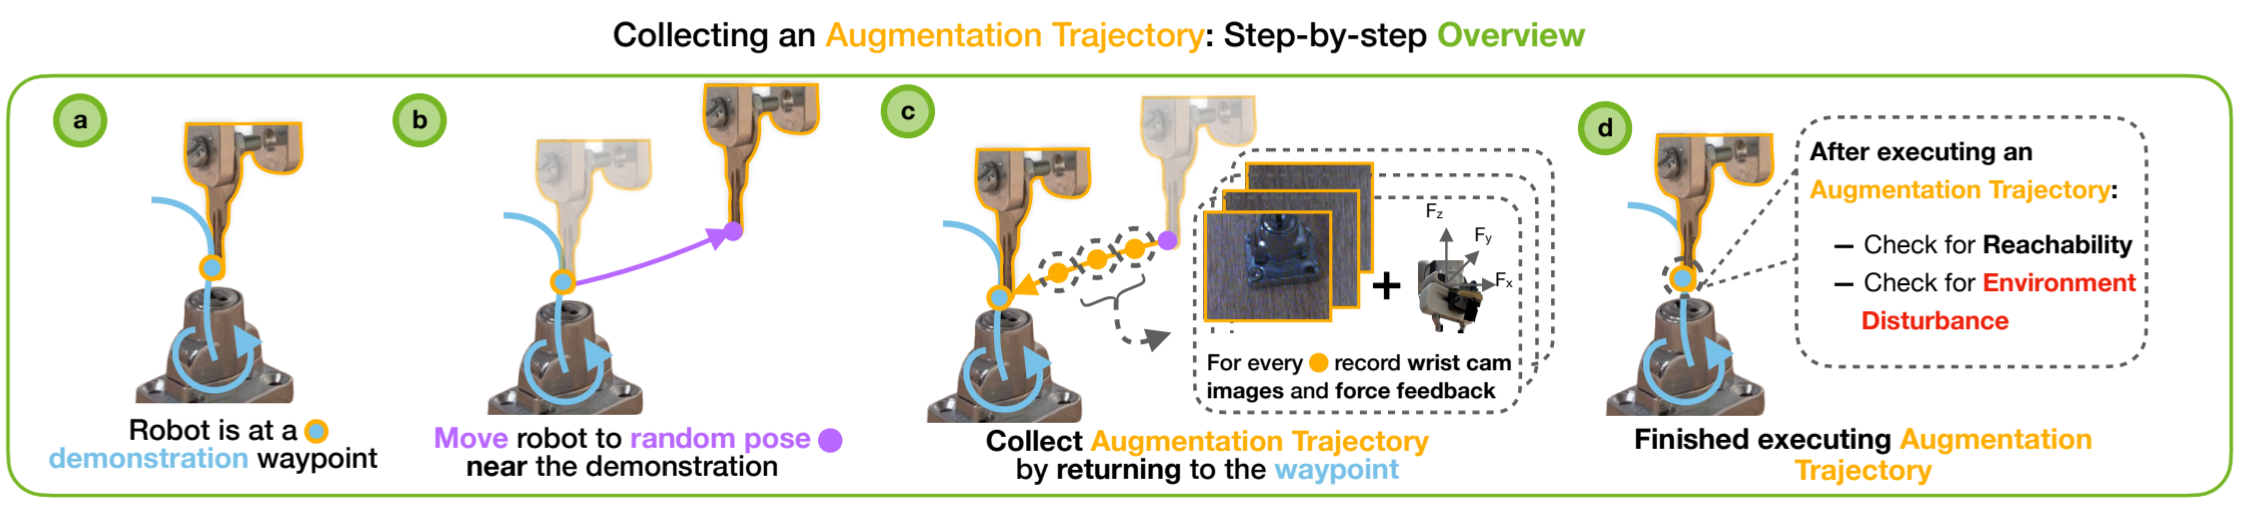
\includegraphics[width=0.7\linewidth]{assets/rel-work/augmentation-miles.png}
  \caption{Process of creating augmented training data \cite{papagiannis2024milesmakingimitationlearning}}\label{fig:aug-miles}
\end{figure}

This is achieved by training a separate policy for each task as a \emph{LSTM} (long-short term memory) network, based on Behavioural Cloning, which is a type of Recurrent Neural Network (RNN) which handles sequential data \cite{medsker2001recurrent}.This allows the policy to learn the gradually changing trajectory while remembering the steps taken in the past. On top of this no object pose priors are given to the network, meaning the networks learnt policies should be applicable to different object poses.

However, another important part of \emph{MILES} is that force sensors are also included in the decision making policies. Which is not a make-or-break addition, as they conclude, the force modality sometimes helps the system achieve better accuracy when coupled with vision, and sometimes not. While just force -without vision, in a somewhat expected manner- performs quite badly in any of the evaluation tasks they have chosen. 



% \cite{natarajan2021graspsynthesisnovelobjects}
\todo[color=green]{this (see comment in file) also kinf of goes under learing using heuristics but not really trajectory maybe move to next section and so some explanation if needed}

\subsection{Attention and Information Gain (IG)}
This is pivotal part of object-centric tasks. Because, if an agent knows what to focus on, then we can teach it a policy to learn to focus on specific subjects.

\subsubsection{\emph{Observe Then Act}}
Taking a third-person-view look to the classical grasping task, \emph{Wang et al.} aim to optimise this viewpoint based on the task goal \cite{wang2024observeactasynchronousactive}. They take a asynchronous viewpoint control approach (see \ref{sec:asynch-synch}); this separation of the camera systems and the motor actions over time. Leading to less need for coordination between the two section and instead, the model focuses more on task-specific movements and distribute this coordination throughout the task. 
They, again, follow a few-shot learning approach. The model comprises of two separate agents, a next-best-view (NBV) agent for optimal viewpoints and next-best-pose (NBP) for determining the gripper's action based on the previous agent's output. Active perceptions is achieved by alternating between sensor and motor action interfaces in each episode; which then leads to the learning of the tasks. These tasks are usually of sequential nature as the asynchronous approach works best with such systems, as they discuss.
\begin{figure}[h]
  \centering
  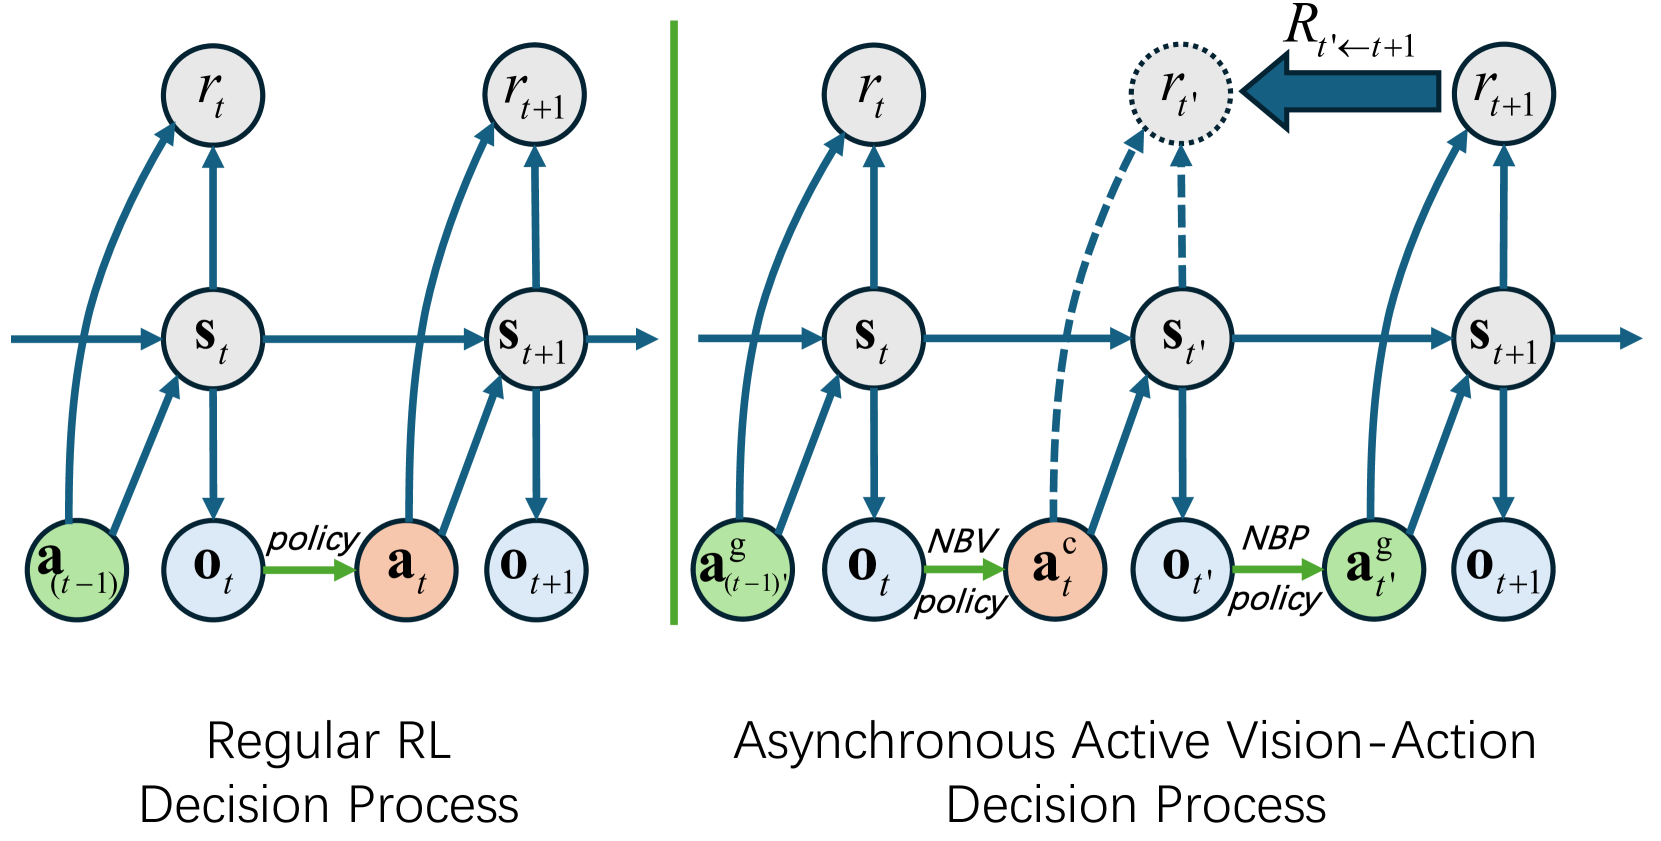
\includegraphics[width=0.5\textwidth]{assets/rel-work/ota-asynch-policy.png}
  \caption{Comparison of regular RL and asynchronous active vision-action decision processes \cite{wang2024observeactasynchronousactive}}\label{fig:oat-neurons}
\end{figure}

They follow a POMDP (\ref{sec:pomdp}) formulation to model the problem:
\(
  \langle \mathcal{O}, \mathcal{A}^c, P, \mathcal{A}^g, \mathcal{O}', P', R, \gamma \rangle
\) where $\mathcal{O}$ and $\mathcal{O}'$ represent the observation spaces at times $t$ and $t'$ the NBV policy $\pi_v$, determines the camera viewpoint action $a_t^c \in \mathcal{A}^c$, given an observation $o_t \in \mathcal{O}$, and obtains a new observation $o_{t'} \in \mathcal{O}'$ through the transition probability $p\left(o_{t'} \mid o_t, a_t^c\right) \in P$. Finally, the NBP policy, $\pi_g$, then determines the gripper action $a^g_{t'} \in \mathcal{A}^g$ based on the new observation $o_{t'}$. then using the transition probability $p'\left(o_{t+1} \mid o_t, a^c_t\right) \in P'$ the next scene observation can be obtained and reward $r_{t+1} \in R$ will be provided. So, the model will be learning these policies: $\pi^*_v$ and $\pi^*_g$ then try to jointly maximise the return for the joint reward for this collective task: 
\[
  \pi_v^*, \pi_g^* = 
  arg~\underset{\pi_v, \pi_g}{max} 
  ~\mathbb{E}
  \left[
    \sum_{t=0}^{\inf}{\gamma^t R(o_t, a^c_t, a^g_t)}
  \right]
\]
\todo[color=green]{more information about the 3D voxels for environment normalisation?? this is more about fighting the caveats of few-shot learning not really fitting here, but might include if it comes in useful later}

Another important contribution here is the use of augmented trajectories again. Similar to \cite{papagiannis2024milesmakingimitationlearning}, demonstration trajectories are augmented in a \emph{viewpoint-aware} manner to expand the learning set by sampling the observations and discovering key frames. It does this while the viewpoint is allowed to shift, meaning the samples getting generated between time frame $T_t$ and $T-{t+1}$ (where $T$ is a trajectory) can have different views, which aids the camera policy in progressive movements. This is done for keyframes for both camera movement and gripper pose, for the two policies.

\subsubsection{Closed-Loop Next-Best-View Planning for Target-Driven Grasping}
Similar in idea, \emph{Breyer et al.} explore yet another grasping task \cite{breyer2022closedloopnextbestviewplanningtargetdriven} (although first-person-view this time) this time. They augment classic grasp synthesis tasks that are mostly reliant on deep learning approaches, which suffer depending on the visual information it has available. Similar to \emph{Wang et al.}, they interact with the environment in an asynchronous manner within a fixed rate. They determine the best candidates for grasping then compute the next-best-view with its associated information gain. 
The information gain metric, allows the system to explore viewpoints in the neighbourhood of the current view and estimate what might be ideal for the grasping, bridging the rewards of the two policies. This again is made possible through the assumption that a task is object dependent hence the model receives bounding boxes and the geometry of the subject of the task.

\begin{figure}[h]
  \centering
  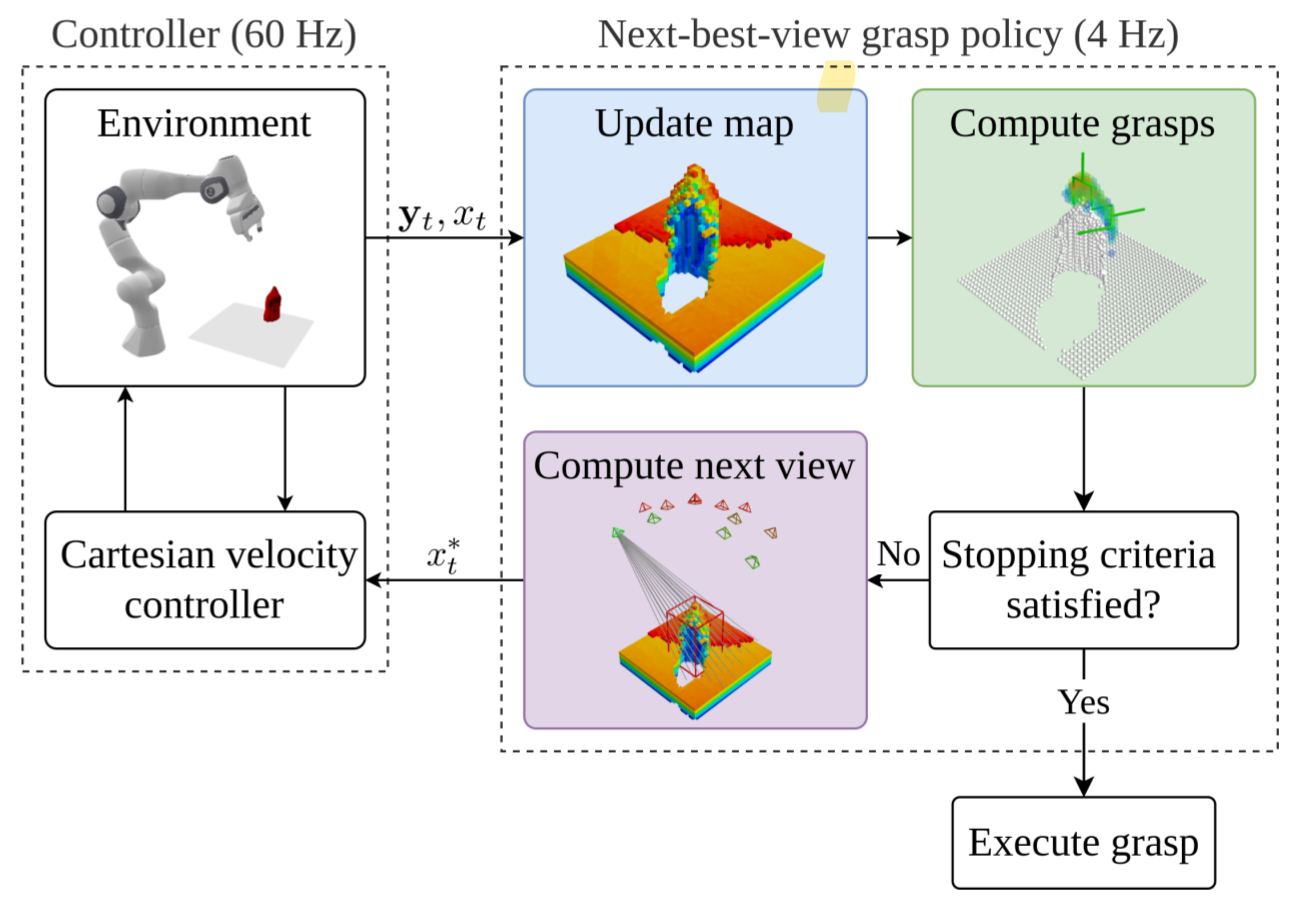
\includegraphics[width=0.4\textwidth]{assets/rel-work/target-grasp.png}
  \caption{How the gripper perceives and finds best poses using object bounding box priors \cite{breyer2022closedloopnextbestviewplanningtargetdriven}}\label{fig:closedloop}
\end{figure}
\todo[color=green]{make a better image for final}

However, the interesting takeaway from their system is an early stopping mechanism. Due to the nature of exploration multiple views can be scanned and many relevant ones can be identified by the system. Without stops, this algorithms may over explore and end up quite inefficient. These stopping conditions include: timeouts (and due to time-framing, limited number of policy updates), minimum thresholding on the information gain so that no unnecessary exploration is done where the estimated IG might be lower; and finally, convergence, when the Volumetric Grasp Network (VGN) \cite{breyer2021volumetricgraspingnetworkrealtime} outputs converge the exploration will stop. 

Therefore, the importance of their research is highlighted in the robustness of their system and the balance they managed to strike between exploration and exploitation. 


\section{Outline}
In summary, work in the field of active vision usually follows an attention metric which is guided by a reward system, usually depending on some priors. The need for priors, although, can be mitigated by providing more demonstrations, this complicates the test setups and operations. Therefore, a common approach is to create augmented data and broaden the horizon of the agent through the exploration of that synthetic space.

Combining these ideas shows us that active vision policy adjustments are not only possible during policy execution but also very promising way to advance the field of robot learning.



%//CHECK interesting paragraph not sure about it tho
% Another interesting point is the relevance of active vision for a task which isn't object-centred. 
% Does the use of active vision make sense to a robot where there isn't a defined subject? Or should the agent explore and find objects of importance?
% \todo{not sure about this paragraph, does this make sense maybe for the final report}